
\ifdefined\COMPLETE
\else
    \input{./preambule-sacha-utf8.ltx}
    \begin{document}
\fi


\setcounter{section}{0} 

\part{Statistique}

\section{Vocabulaire}

\begin{tabular}{c|c|c}

Vocabulaire ensembliste & Vocabulaire statistique & Vocabulaire probabiliste \\
\hline
Ensemble & Population & Univers \\
Sous-ensemble & Échantillon & Événement \\
Élément & Individu & Éventualité (cas possible) \\
Propriété & Caractère & {\Large $\times$} \\
\end{tabular} \\

% \textbf{Exemple} \\

\begin{center}

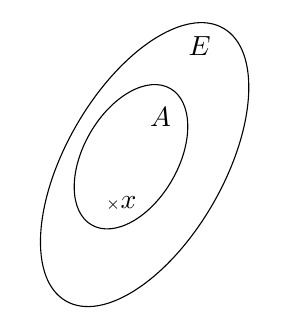
\begin{tikzpicture}
\begin{scope} [rotate=-30]
\draw (0,0)  circle  (1 and 2); 
\draw (0,0) ++(0:-.2) circle (.6 and 1); 
\end{scope} 
\draw (0.7,1.5) node {$E$} ; 
\draw (.2,.6) node {$A$} ; 
\draw (-.3,-.5) node {{\tiny $\times$} $\!\!x$} ; 
\end{tikzpicture}

$ A \subset E $, car A est un sous-ensemble de E.

$ x \in A $ et $ x \in E $ car $x$ est un élément de A, et par conséquent un élément de E. \\

\vspace*{2cm}


Il existe différents types de caractères : \\

\bigskip 
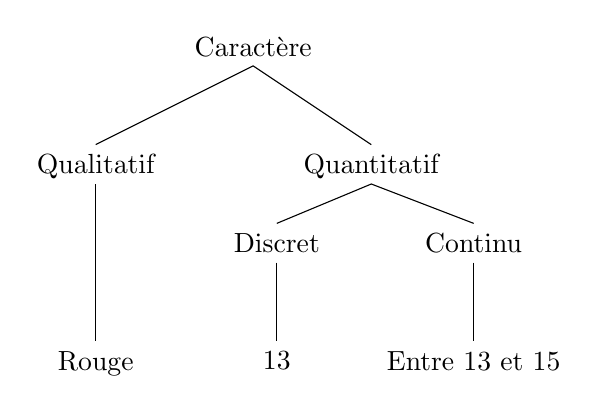
\begin{tikzpicture}
\draw(-2,2) node [below] {Qualitatif} -- (0,3) node [above] {Caractère} 
-- (1.5,2) node [below] {Quantitatif} ; 
\draw (-2,1.5) -- (-2,-.5) node [below] {Rouge} ; 
\draw (0.3,1) node [below]{Discret} -- (1.5,1.5) -- (2.8,1) node [below]{Continu} ; 
\draw (0.3,.5) -- (0.3,-.5) node [below]{13} ; 
\draw (2.8,.5) -- (2.8, -.5) node [below]{Entre 13 et 15} ; 
\end{tikzpicture}
\end{center} 

\newpage

\vspace*{-2cm}

\section{Caractéristiques d'une série statistique}

Soit $\left(x_i \; ; \; n_i \right)$ une série statistique, dont le caractère étudié est le nombre de frères et sœurs. \\

\begin{tabular}{c|c}
Valeur du caractère $x_i$ & Effectifs $n_i$ \\
\hline
$0$ & $3$ \\
$1$ & $7$ \\
$2$ & $10$ \\
$3$ & $5$ \\
$4$ & $2$ \\
$5$ & $1$ \\
\hline
$\Sigma$ & $28$ \\
\end{tabular}

\vspace*{.3cm}

On lit que $x_2 = 1$ ; $n_1 = 3$ et $n_6 = 1$. \\

On a $\Sigma_{n_i} = 28 = n_1 + n_2 + n_3 + n_4 + n_5 + n_6$ 

\subsection{Le mode}

Le mode est la  valeur du caractère qui a le plus grand effectif. \\

\textbf{Exemple}

Les modes de la série statistique de la série précédente est $2$.

\subsection{L'étendue}

C'est la différence entre la plus grande valeur et la plus petite valeur du caractère. \\

\textbf{Exemple}

Dans la série statistique de la série précédente, l'étendue est $5 - 0 = 5$.

\subsection{La médiane}

Si elle existe, la médiane est la valeur du caractère qui partage l'effectif total en deux parties de même effectif. \\

\textbf{Exemple n°1}

Notes classées par ordre croissant. \\

$ \underbrace{ 7 \, ; \,  8 \, ; \,  9 \, ; \,  9 \, ; \,  10 \, ; \,  10 \, ; \, } 11 \underbrace{\, ; \,  12 \, ; \,  13 \, ; \,  14 \, ; \,  14 \, ; \,  15 \, ; \,  17.} $ \\

$ N = \Sigma_{n_i} = 13$ \\

$N$ est impair. La médiane est donc le terme de rang $\dfrac{N+1}{2}$. 

Donc $med = 11$ \\

\textbf{Exemple n°2} \\

$ \underbrace{7 \, ; \,  7 \, ; \,  9 \, ; \,  9 \, ; \,  10 \, ; \,  11 \, ; \, } 12 \, ; \,  13 \underbrace{\, ; \,  13 \, ; \,  13 \, ; \,  14 \, ; \,  14 \, ; \,  15 \, ; \,  15.}$ \\

$ N = 14 $. \\

$N$ est pair. La médiane est donc la moyenne entre le terme de rang $\dfrac{N}{2}$ et celui de rang $\dfrac{N}{2} + 1$. \\
Donc $med = \dfrac{12 + 13}{2} = 12,5 $. 

\newpage

\subsection{Les quartiles}

\begin{itemize}
\item[*] Le premier quartile $Q_1$ est la plus petite valeur du caractère telle qu'au moins 25\% des valeurs du caractère soient inférieures ou égales à ce nombre.
\item[*] Le troisième quartile $Q_3$ est la plus petite valeur du caractère telle qu'au moins 75\% des valeurs du caractère soient inférieures ou égales à ce nombre.
\end{itemize}

\vspace*{.3cm}

\textbf{N.B.} : Le deuxième quartile n'est autre que la médiane.

\vspace*{.3cm}

\textbf{Exemple n°1} \\

$ 7 \, ; \,  7 \, ; \,  8 \, ; \,  9 \, ; \,  10 \, ; \,  12 \, ; \,  13 \, ; \,  13 \, ; \,  15 \, ; \,  16 \, ; \,  17 \, ; \,  18.$ \\

$\Sigma_{n_i} = N = 12$ \\

$N$ est divisible par 4. Donc $Q_1$ est le terme de rang $\dfrac{N}{4}$, et $Q_3$ est le terme de rang $\dfrac{3N}{4}$. \\

Ainsi,  \\

\begin{itemize}
\item[*] $\dfrac{N}{4} = 3$, donc $Q_1 = 8$.
\\
\item[*] $ \dfrac{3N}{4} = 9$, donc $Q_3 = 15$.
\end{itemize}

\vspace*{.3cm}

\textbf{Exemple n°2} \\

$ 7 \, ; \,  7 \, ; \,  8 \, ; \,  9 \, ; \,  10 \, ; \,  12 \, ; \,  13 \, ; \,  13 \, ; \,  15 \, ; \,  16 \, ; \,  17 \, ; \,  18 \, ; \,  19.$ \\

$\Sigma_{n_i} = N = 13$ \\

$N$ n'est pas divisible par 4. Donc $Q_1$ est le terme de rang le premier nombre entier qui suit $\dfrac{N}{4}$, 

et $Q_3$ est le terme de rang le premier nombre entier qui suit $\dfrac{3N}{4}$. \\

Ainsi,  \\

\begin{itemize}
\item[*] $\dfrac{N}{4} = 3,25$, donc $Q_1$ est le terme de rang 4, et $Q_1 = 9$.
\\
\item[*] $ \dfrac{3N}{4} = 9,75$, donc $Q_3$ est le terùe de rang 10, et $Q_3 = 16$.
\end{itemize}

\newpage

\textbf{On peut aussi faire des tableaux :}

%Y mettre les couleurs. J'ai écrit la légende...

En orange l'« affichage machine », en rouge les quartiles et en vert la médiane. \\

Sur l'exemple n°1 : \\

\begin{itemize}
\item[*] Médiane : $N$ est pair. On a $\dfrac{N}{2} = 6$ et $\dfrac{N}{2} + 1 = 7$. D'où $med = \dfrac{12 + 13}{2} = 12,5$. \\
\item[*] Quartiles : $N$ est divisible par $4$. On a $\dfrac{N}{4} = 3$, et $\dfrac{3N}{4} = 9$. D'où $Q_1 = 8$ et $Q_3 =15$. \\
\end{itemize}

\begin{tabular}{rrc|c|c}
& & $x_i$ & $n_i$ & Effectifs cumulés croissants \\
\cline{3-5}
\textcolor{DarkOrange}{$\mathrm{min}_{x}$}&   & 7 & 2 & 2 \\
\textcolor{DarkOrange}{$Q_1 = 8.5$}& \textcolor{Red}{$Q_1$}
    & 8 & 1 & $\quad$ 3 \textcolor{red}{$\leftarrow$}\\
& & 9 & 1 & 4 \\
& & 10 & 1 & 5 \\
% Les accollades par paire sinon le vert déteint
& \multirow{2}{2cm}{{\color{VertClair}
 $\left. \begin{array}{c}
          \mathrm{\fcolorbox{red}{white}{med=12.5}}\\
          \end{array}
  \right[$
 } }                  & 12 & 1 
           & $\quad$ 6 \textcolor{VertClair}{$\leftarrow$} \\
& & 13 & 2 & $\quad$ 8 \textcolor{VertClair}{$\leftarrow$}  \\
\textcolor{DarkOrange}{$Q_3 = 15.5$}
    &  \textcolor{Red}{$Q_3$}& 15 & 1 & $\quad$ 9 \textcolor{red}{$\leftarrow$} \\
& & 16 & 1 & 10 \\
& & 17 & 1 & 11 \\
\textcolor{DarkOrange}{$\mathrm{max}_x$}& & 18 & 1 & 12 \\
\cline{3-5}
& &  $\Sigma$ & 12 & {\Large $\times$} \\
& &  &\textcolor{DarkOrange}{n}& \\
\end{tabular}

\vspace*{.5cm}

Sur l'exemple n°2 : \\

\begin{itemize}
\item[*] Médiane : $N$ est impair. On a $\dfrac{N+1}{2} = 7$ D'où $med = 13$. \\
\item[*] Quartiles : $N$ n'est pas divisible par $4$. On a $\dfrac{N}{4} = 3,25$, et $\dfrac{3N}{4} = 9,75$. \vspace*{.3cm} \\ D'où $Q_1$ est le $4^{\mathrm{ème}}$ terme et $Q_1 = 9$ et $Q_3$ est le $10^{\mathrm{ème}}$ terme et $Q_3 =16$. \\
\end{itemize}

\begin{tabular}{rrc|c|c}
&&$x_i$ & $n_i$ & Effectifs cumulés croissants \\
\cline{3-5}
\textcolor{DarkOrange}{$\mathrm{min}_{x}$} & & 7 & 2 & 2 \\
&&8 & 1 & 3 \\
\textcolor{DarkOrange}{$Q_1 = 8.5$}& \textcolor{Red}{$Q_1$}
       & 9 & 1 & $\quad$ 4 \textcolor{red}{$\leftarrow$} \\
&&10 & 1 & 5 \\
&&12 & 1 & 6 \\
&\textcolor{VertClair}{med} & \fcolorbox{red}{white}{13} 
     & 2 & $\quad$ 8 \textcolor{VertClair}{$\leftarrow$}  \\
&&15 & 1 & 9 \\
\textcolor{DarkOrange}{$Q_3 = 15.5$}
    &  \textcolor{Red}{$Q_3$} & 16 & 1 
            &  $\quad$ 10 \textcolor{red}{$\leftarrow$} \\
&&17 & 1 & 11 \\
&&18 & 1 & 12 \\
\textcolor{DarkOrange}{$\mathrm{max}_x$}&&19 & 1 & 13 \\
\cline{3-5}
&&$\Sigma$ & 13 & {\Large $\times$} \\
& &  &\textcolor{DarkOrange}{n}& \\
\end{tabular}

\newpage

\subsection{Diagramme en boîte (ou boîte à moustaches)}

\textbf{Exemple n°1 :}

%Mettre le dessin.
 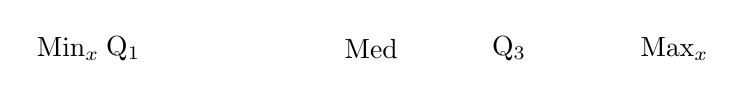
\begin{tikzpicture}[scale=0.7]
\tkzInit[xmax=20,xstep=1,ymax=2]
\tkzGrid [ultra thin,
% color=AntiqueWhite!10,sub,
color=AntiqueWhite,sub,
%       subcolor=AntiqueWhite!20,
       subxstep = 1](0,0)(20,2)
% \tkzLabelX[orig=false, color=white]
\tkzLabelX 
\tkzWhbox{7,8,12.5,15,18}
\draw (7,-1) node{$\mathrm{Min}_{x}$} ;  
\draw (8,-1) node{$\mathrm{Q}_{1}$} ;  
\draw (12.5,-1) node{Med} ; 
\draw (15,-1) node{$\mathrm{Q}_{3}$} ;   
\draw (18,-1) node{$\mathrm{Max}_{x}$} ;  
\end{tikzpicture}

\vspace*{.3cm}

L'écart inter-quartile est $Q_3 - Q_1 = 15 - 8 = 7$. \\ C'est la longueur de la boîte.

% \bigskip

\textbf{Exemple n°2 :}

%Mettre le dessin.
 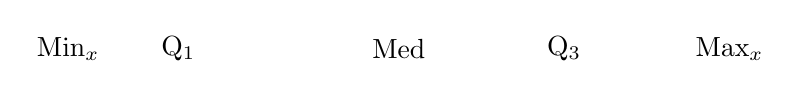
\begin{tikzpicture}[scale=0.7]
\tkzInit[xmax=20,xstep=1,ymax=2]
\tkzGrid [ultra thin,
% color=AntiqueWhite!10,sub,
color=AntiqueWhite,sub,
%       subcolor=AntiqueWhite!20,
       subxstep = 1](0,0)(20,2)
% \tkzLabelX[orig=false, color=white]
\tkzLabelX 

\tkzWhbox{7,9,13,16,19}
\draw (7,-1) node{$\mathrm{Min}_{x}$} ;  
\draw (9,-1) node{$\mathrm{Q}_{1}$} ;  
\draw (13,-1) node{Med} ; 
\draw (16,-1) node{$\mathrm{Q}_{3}$} ;   
\draw (19,-1) node{$\mathrm{Max}_{x}$} ;  

\end{tikzpicture}

L'écart inter-quartile est $Q_3 - Q_1 = 16 - 9 = 7$. \\ C'est la longueur de la boîte. \\

\textbf{À la calculatrice :} \\

Rentrer les valeurs dans les colonnes $L1$ pour les $x_i$ et $L2$ pour les $n_i$, en appuyant sur « stats » \\ puis « 1: Edite ». \\
Après que les valeurs aient été entrées, appuyer sur « stats » puis aller dans l'onglet « CALC ». \\ Appuyer sur « 1: Stats 1 - Var », puis entrer « L1,L2 » (les touches L1 et L2 sont accessibles \\ par l'intermédiaire de la touche « 2nde »). On peut donc vérifier ses résultats. \\

\underline{Pour la boite à moustaches}, faire « 2nde » puis « f(x) » pour activer la fonction « graph stats ». \\ Puis « Entrer » pour choisir le premier Graph, et choisir en-dessous celui qui ressemble à une \\ boite à moustaches, le deuxième de la deuxième ligne. \\

Enfin, appuyer sur « fenêtre », la définir, puis « graphe » pour tracer la boîte à moustaches. 

\subsection{La moyenne}

Soit $\left(x_i \; ; \; n_i\right)$ une série statistique. \\ 

\begin{tabular}{c|c|c}
$x_i$ & $n_i$ & $n_ix_i$ \\
\hline
2 & 2 & 4	\\
6 & 7 & 42 \\
10 & 9 & 90 \\
14 & 9 & 126 \\
18 & 1 & 18 \\
\hline
$\Sigma$ & 28 & 280 \\
    & \textcolor{DarkOrange}{n} & \textcolor{DarkOrange}{$\Sigma x$} \\
\end{tabular}

\vspace{.3cm}

$\overline{x} = \dfrac{\Sigma_{n_ix_i}}{\Sigma_{n_i}} $ \\

$\overline{x} = \dfrac{280}{28} = 10 $

\newpage

\subsection{L'écart type}

\textbf{a) Introduction}

On observe les résultats en mathématique de 2 élèves, Sylvain et Sylvette, au cours d'un trimestre. On appelle « Élève A » Sylvain, et « Élève B », Sylvette. \\

\begin{itemize}
\item[*] Élève A : $ 11 / 9 / 13 $
\item[*] Élève B : $ 12 / 3 / 18 $
\end{itemize}

\vspace{.3cm}

On constate que $\overline{x_A} = \overline{x_B} = 11 $. \\

\centerline{\footnotesize
\begin{tabular}{c|c|c|c|c|c|c|c|c|c}
& Notes & Moyenne & Écarts & Moyenne & Valeurs & Moyenne & Carrés & Moyenne & Racine \\ 
& & & par & des & absolues & des & des & des & carrée \\
& & & rapport & écarts & des & valeurs & écarts & carrés & de la \\
& & & à la & par & écarts & absolues & par & des & moyenne \\
& & & moyenne & rapport & par & des & rapport & écarts & des \\
& & & & à la & rapport & écarts & à la & par & carrés \\
& & & & moyenne & à la & par & moyenne & rapport & des \\
& & & & & moyenne & rapport & & à la & écarts \\
& & & & & & à la & & moyenne & par \\
& & & & & & moyenne & & & rapport \\
& & & & & & & & & à la \\
& & & & & & & & & moyenne \\
\hline
& & & & & & & & & \\
Élève A & $11$ / $9$ / $13$ & $11$ & $0$ / $-2$ / $+2$ & $0$ & $0$ / $2$ / $2$ & $\dfrac{4}{3} \approx 1,33$ & $0$ / $4$ / $4$ & $\dfrac{8}{3} \approx 2,67$ & $\sqrt{\dfrac{8}{3}} \approx 1,63$ \\
& & & & & & & & & \\
Élève B & $12$ / $3$ / $18$ & $11$ & $+1$ / $-8$ / $+7$ & $0$ & $1$ / $8$ / $7$ & $\dfrac{16}{3} \approx 5,33$ & $1$ / $64$ / $49$ & $38$ & $\sqrt{38} \approx 6,16$ \\
%& & & & RATÉ, il aurait fallu faire une moyenne arithmétique, pas algébrique & & Pas mal, mais pas exploitable & & Ça n'a pas de signification, des points au carré & \\
\hline
& & & & & & & & & \\
& & & & & & & ÉCART-MOYEN & VARIANCE & ÉCART-TYPE \\
\end{tabular}}

\vspace*{.5cm}

\textbf{b) Définition :}

On note l'écart type $\sigma_x$, et on a : $ \sigma_x = \sqrt{\dfrac{\Sigma_{n_i}\left(x_i - \overline{x}\right)^2}{\Sigma_{n_i}}} $. \\

\textbf{c) Exemple :} \\

\begin{tabular}{c|c|c|c}
$x_i$ & $n_i$ & $n_ix_i$ & $n_i\left(x_i - \overline{x}\right)^2$ \\
\hline
2 & 2 & 4 & 128 	\\
6 & 7 & 42 & 112 \\
10 & 9 & 90 & 0 \\
14 & 9 & 126 & 144 \\
18 & 1 & 18 & 64 \\
\hline
$\Sigma$ & 28 & 280 & 448 \\
\end{tabular}

\vspace*{.3cm}

$ \overline{x} = \dfrac{\Sigma{n_ix_i}}{\Sigma_{n_i}} = \dfrac{280}{28} = 10 $ \\

\vspace*{.3cm}

$\sigma_x = \sqrt{\dfrac{448}{28}} = 4 $ \\

\newpage

\vspace*{-1cm}

\textbf{d) Autre formule} \\

$ \sigma_x^2 = \dfrac{\Sigma_{n_i \times \left(x_i - \overline{x}\right)^2}}{\Sigma_{n_i}} $ \\

$ \sigma_x^2 = \dfrac{\Sigma_{n_i \left(x_i^2 - 2\overline{x}x_i + \overline{x}^2\right)}}{\Sigma_{n_i}} $ \\

$ \sigma_x^2 = \dfrac{\Sigma_{n_ix_i^2 - 2n_ix_i\overline{x} + n_i\overline{x}^2}}{\Sigma_{n_i}} $ \\

$ \sigma_x^2 = \dfrac{\Sigma_{n_ix_i^2} - 2\overline{x}\Sigma_{n_ix_i} + \overline{x}^2\Sigma{n_i}}{\Sigma_{n_i}} $ \\

$ \sigma_x^2 = \dfrac{\Sigma_{n_ix_i^2}}{\Sigma_{n_i}} - 2\overline{x} \dfrac{\Sigma_{n_ix_i}}{\Sigma_{n_i}} + \overline{x}^2 \dfrac{\Sigma_{n_i}}{\Sigma_{n_i}} $ \\

$ \sigma_x^2 = \overline{x^2} - 2\overline{x} \times \overline{x} + \overline{x}^2 \times 1 $ \\

$ \sigma_x^2 = \overline{x^2} - 2\overline{x}^2 + \overline{x}^2 $ \\

$ \sigma_x^2 = \overline{x^2} - \overline{x}^2 $

Et donc $ \sigma_x = \sqrt{\overline{x^2} - \overline{x}^2} $ \\

\textbf{e) Exemple :} \\

\begin{tabular}{c|c|c|c}
$x_i$ & $n_i$ & $n_ix_i$ & $n_ix_i^2$ \\
\hline
2 & 2 & 4 & 8 	\\
6 & 7 & 42 & 252 \\
10 & 9 & 90 & 900 \\
14 & 9 & 126 & 1764 \\
18 & 1 & 18 & 324 \\
\hline
$\Sigma$ & 28 & 280 & 3248 \\
\end{tabular}

\vspace{.3cm
}
On rappelle que $\overline{x} = 10 $. \\

On a : $ \sigma_x = \sqrt{\overline{x^2} - \overline{x}^2} = \sqrt{\dfrac{3248}{28} - \left(\dfrac{280}{28}\right)^2} = 4 $ \\

%On notera l'affiche machine en orange...

On peut vérifier à la calculatrice : 

\begin{itemize}
\item[*] $\overline{x} = 10$ 
\item[*] $\Sigma_x = 280$ 
\item[*] $\Sigma_{x^2} = 3248$ 
\item[*] $\sigma_x = 4$ 
\item[*] $n = 28$ 
\item[*] $min_x = 2$ 
\item[*] $Q_1 = 6$ 
\item[*] $Med = 10$ 
\item[*] $Q_3 = 14$ 
\item[*] $max_x = 18$ \\
\end{itemize}

Elle nous donne tout ! \vspace*{.3cm}

Néanmoins, il faut faire attention aux valeurs des quartiles données par la calculatrice... \\ Elles sont à prendre avec des pincettes !

\vspace*{-5cm}

\newpage

\subsection{Répartition « normale »}

Soit $\left(x_i,n_i\right)$ une série statistique. 

Soient $\overline{x}$ la moyenne et $\sigma_x$ l'écart-type. \\

On considère que la répartition est « normale » : \\

\begin{itemize}
\item[*] si les valeurs du caractère comprises entre $\overline{x} - \sigma_x$ et $\overline{x} + \sigma_x$ représentent 68\% de l'effectif total.
\item[*] \textbf{ou} si les valeurs du caractère comprises entre $2\overline{x} - 2\sigma_x$ et $2\overline{x} + 2\sigma_x$ représentent 95\% de l'effectif total.
\item[*] \textbf{ou} si les valeurs du caractère comprises entre $3\overline{x} - 3\sigma_x$ et $3\overline{x} + 3\sigma_x$ représentent 99\% de l'effectif total.
\end{itemize}

\vspace*{.3cm}

%Mettre les dessin.

\pgfmathdeclarefunction{gauss}{2}{%
    \pgfmathparse{1/(#2*sqrt(2*pi))*exp(-((x-#1)^2)/(2*#2^2))}%
        }

\begin{tikzpicture}

    \begin{axis}[
      hide y axis, tick align=outside,
      domain=-4:4, samples=50,
%       axis lines*=left, xlabel=Gauss, ylabel=$~$,
        axis lines*=left, xlabel=$~$, ylabel=$~$,
      height=5cm, width=13cm,
      xtick={-4,-3,-1.5,-1,0,1,1.5,3,4}, ytick=\empty,
      xticklabels={%
        $\overline{x}-3\sigma_x$,
        $\overline{x}-2\sigma_x$,
        $\overline{x}-\sigma_x$,
        ,
        $\overline{x}$,
        ,
        $\overline{x}+\sigma_x$,
        $\overline{x}+2\sigma_x$,
        $\overline{x}+3\sigma_x$}      
      ]
   
      \addplot [fill=blue!30, domain=-1.5:1.5] {gauss(0,1)}\closedcycle;
         
            \addplot [thick,red,domain=-4:4] {gauss(0,1)};
   \addplot [red, domain=-4:4] {gauss(0,1)}\closedcycle;
   
         \addplot [thick,green,domain=-3:3] {gauss(0,1)};
      \addplot [fill=VertClair, domain=-3:-1.5] {gauss(0,1)}\closedcycle;   
      \addplot [fill=VertClair, domain=1.5:3] {gauss(0,1)}\closedcycle;

      \addplot [thick,black!50!black,domain=-1.5:1.5] {gauss(0,1)};

    \end{axis}
    
    \draw (5.7,1.5) node {68\%} ;  
    \draw [VertClair](10,3) node {$\bumpeq \; $ 95\%} ;    
    \draw [red](10,2.5) node {$\bumpeq \; $ 99\%} ; 
\end{tikzpicture}

Ceci est appelé « Courbe en cloche de Gauss ». \\

\textbf{Exemple} \\

Si $\overline{x} = 10$ et $ \sigma_x = 4$, alors : \\

\begin{itemize}
\item[*] $\overline{x} - \sigma_x = 6$ et $\overline{x} + \sigma_x = 14$. On a donc $7 + 9 + 9 = 25$ élèves, soit 89,3\%. \\
\item[*] $2\overline{x} - 2\sigma_x = 2$ et $2\overline{x} + 2\sigma_x = 18$. On a donc $28$ élèves, soit 100\%. 
\end{itemize}

\newpage

\section{Exercice : Étude d'un caractère quantitatif discret}

Dans une maternité, on étudie la taille des bébés en cm pour 200 bébés. \\

\begin{tabular}{rc|c|c|c|c|c}
&\textcolor{DarkOrange}{\Ovalbox{$L_1$}}
          &\textcolor{DarkOrange}{\Ovalbox{$L_2$}}&&&&\\
 & $x_i$ & $n_i$ & $p_i$ & Effectifs cumulés croissants & $n_ix_i$ & $n_ix_i^2$ \\
\cline{2-7}
 \textcolor{DarkOrange}{$\mathrm{min}_{x}$} & 43 & 4 & 2 & 4 & 172 & 7 396 \\
 & 44 & 0 & 0 & 4 & 0 & 0 \\
 & 45 & 0 & 0 & 4 & 0 & 0 \\
 & 46 & 8 & 4 & 12 & 368 & 16 928 \\
 & 47 & 16 & 8 & 28 & 752 & 35 344 \\
 & 48 & 22 & 11 & 50 & 1056 & 50 688 \\
 & 49 & 38 & 19 & 88 & 1862 & 91 238 \\
 & 50 & 42 & 21 & 130 & 2100 & 105 000 \\
 & 51 & 30 & 15 & 160 & 1530 & 78 030 \\
 & 52 & 16 & 8 & 176 & 832 & 43 264 \\
 & 53 & 14 & 7 & 190 & 742 & 39 326 \\
 & 54 & 4 & 2 & 194 & 216 & 11 664 \\
 & 55 & 4 & 2 & 198 & 220 & 12 100 \\
 & 56 & 0 & 0 & 198 & 0 & 0 \\
 \textcolor{DarkOrange}{$\mathrm{max}_{x}$} & 57 & 2 & 1 & 200 & 114 & 6 498 \\
\cline{2-7}
 & $\Sigma$ & 200 & 100 & {\Large $\times$} & 9 964 & 497 476 \\
 &  & \textcolor{DarkOrange}{n} &\multicolumn{2}{c}{}   
 & \multicolumn{1}{c}{\textcolor{DarkOrange}{$\Sigma x$} } 
 &  \multicolumn{1}{c}{\textcolor{DarkOrange}{$\Sigma x^2$}}\\ 
\end{tabular}

\subsection{Mode et étendue}

\begin{itemize}
\item[*] Mode : $50$
\item[*] Etendue : $57 - 43 = 14$.
\end{itemize}

\medskip 

\begin{center}
\textbf{Diagramme en bâtons des pourcentages}

\begin{tikzpicture}[scale=.7]
    \tkzInit[xmin=42,xmax=57,ymax=22, ystep=2]

    \tkzGrid[color=AntiqueWhite]
    \tkzDrawX[label=$~$]
    \tkzLabelX[orig=false, color=black ]
   \tkzDrawY[label=$~$]
    \tkzLabelY[orig=false]
%     \tkzAxeXY
    \tkzBardiagram[wd = 0.1,
                   pos = {below,outer sep = 5pt},
                   sp = 1,
                   noval]
     { /2, /0, /0, /4, /8, /10.5, /19, /21, /17, /8, /7, /2, /2, /0, /1}
%            \draw (13,9) node{\large Diagramme en bâtons des effectifs} ;  
\end{tikzpicture}
\end{center}

\newpage 

\subsection{Médiane, 1$^{\mathrm {\bf er}}$ quartile et 3$^{\mathrm{\bf e}}$ quartile}

\textbf{Médiane} \\

$ N = 200 $. $N$ est un nombre pair. \\

$\dfrac{N}{2} = 100 $ et $\dfrac{N}{2} + 1 = 101 $. \\

\begin{itemize}
\item[*] Le terme de rang 100 est 50.
\item[*] Le terme de rang 101 est 50.
\end{itemize}

\vspace*{.3cm}

$\mathrm{med} = \dfrac{50 + 50}{2} = $ 
      \textcolor {DarkOrange}{\Ovalbox {\textcolor{black}{50}} med = 50}. \\

$\mathbf{Q_1}$ \textbf{et} $\mathbf{Q_3}$ \\

$ N = 200 $. $N$ est divisible par 4. \\

$\dfrac{N}{4} = 50 $ et $\dfrac{3N}{4} = 150 $. \\

\begin{itemize}
\item[*] Le terme de rang 50 est 48.
\item[*] Le terme de rang 150 est 51.
\end{itemize}

\vspace*{.3cm}

Donc $Q_1 = 48$ et $Q_3 = 51$. \\

\textbf{Boîte à moustaches}

\bigskip 

%Inclure le dessin.

 \begin{tikzpicture}[scale=0.7]
\tkzInit[xmin=42,xmax=58,xstep=1,ymax=2]
\tkzGrid [ultra thin,
% color=AntiqueWhite!10,sub,
color=AntiqueWhite,sub,
%       subcolor=AntiqueWhite!20,
       subxstep = 1](42,0)(58,2)
% \tkzLabelX[orig=false, color=white]
\tkzLabelX 

\tkzWhbox{43,48,50,51,57}
\draw (1,1.5) node{$\mathrm{Min}_{x}$} ;  
\draw (5.5,1.5) node{$\mathrm{Q}_{1}$} ;  
\draw (8,1.8) node{Med} ; 
\draw (9.5,1.5) node{$\mathrm{Q}_{3}$} ;   
\draw (15,1.5) node{$\mathrm{Max}_{x}$} ;  

\end{tikzpicture}

Interprétation de la médiane : \\

Environ 50\% des bébés mesurent moins de 50 cm. \\
Environ 50\% des bébés mesurent plus de 50 cm. \\

Interprétation de l'\underline{écart interquartile} : \\

Environ 50\% des bébés mesurent entre 48 et 51 cm. 

\subsection{Moyenne et écart-type}

$\overline{x} = \dfrac{\Sigma_{n_ix_i}}{\Sigma_{n_i}} = \dfrac{9964}{200} = 49,82$. \\

Donc $\overline{x} = 49,82$cm. \\

$\sigma_x = \sqrt{\overline{x^2} - \overline{x}^2} = \sqrt{\dfrac{497476}{200} - \left(\dfrac{9964}{200}\right)^2} \approx 2,31$. \\

Donc $\sigma_x = 2,31$cm. \\

\subsection{Répartition « normale »}

\begin{itemize}
\item[*] $\overline{x} - \sigma_x = 47,51$. \\ $\overline{x} + \sigma_x = 52,13$. \\On a donc $22 + 38 + 42 + 30 + 16 = 148$ bébés, soit 74\%. 
\\
\item[*] $\overline{x} - 2\sigma_x = 45,20$ \\ $\overline{x} + 2\sigma_x = 54,44$. \\ On a donc $200 - 4 - 4 - 2 = 190$ bébés, soit 95\%. 
\end{itemize}

\ifdefined\COMPLETE
\else
    \end{document}
\fi